\chapter{Fundamentação Teórica}
\label{cap:fund}

% figuras estão no subdiretório "figuras/" dentro deste capítulo
\graphicspath{\currfiledir/figuras/}


\section{Redes Sociais}

\begin{itemize}
\item Histórico de redes sociais
\item Tipos de redes sociais
\item Redes parecidas com nosso trabalho
\item Análises de tempo despendido em redes sociais.
\end{itemize}

Desde a invenção da internet em 1991, mais e mais aplicações vem sendo criadas para facilitar e estimular os relacionamentos virtuais. As redes sociais virtuais tiveram início em 1997 com o site \emph{Six Degrees}, \citep{terrel17}. \emph{Six Degrees} é nomeado em referência ao estudo de \cite{milgram67}, que teorizava que são necessários seis laços de amizade para que quaisquer pessoas estejam conectadas. \emph{Six Degrees} teve seu fim em 2001, mas iniciou o processo de popularização das redes sociais e é considerado a primeira rede social pois permitia que as pessoas criassem seus perfis individuais e adicionar outros contatos à sua rede. Teve 3,5 milhões de usuários no seu auge.

Entre as precursoras está também a rede especializada em relacionamentos profissionais, \emph{LinkedIn}. Foi criada em no final de 2002 e tem, desde então, seu objetivo principal em criar conexões entre profissionais, estudantes e corporações. O \emph{LinkedIn} é, ainda hoje, a rede mais popular neste nicho com mais de 500 milhões de usuários.

A rede mais popular atualmente, segundo \cite{lua19}, é o Facebook com 2,23 milhões de usuários ativos mensalmente. O Facebook foi criado em 2004 como uma rede específica para estudantes da Universidade de Harvard. Em 2006 foi aberta ao público e em 2008 já era a rede social mais visitada do mundo.

Há também redes especializadas em outros tipos de conexão ou outras maneiras de publicar conteúdo. O YouTube é uma rede social especializada na divulgação de vídeos criados pelos usuários. O Twitter, distingue-se das outras redes por iniciar suas atividades permitindo apenas a publicação de textos com, no máximo, 140 caracteres. Este limite foi dobrado posteriormente, mas o foco ainda mantém-se em pequenas postagens.

Por fim, há as redes especializadas em relacionamentos românticos. O Tinder, o Happn e o OKCupid são exemplos de redes sociais direcionadas à criação de relacionamentos íntimos entre os usuários. O sistema desenvolvido neste trabalho enquadra-se nesta categoria pois tem o objetivo de colocar usuários em contato com pessoas desconhecidas que têm potencial para formarem amizades ou até mesmo casais.

No Brasil, 66\% da população tem acesso à internet segundo \cite{wearesocial18}. Dentre os usuários da internet 93\% são ativos em alguma rede social.
Segundo \cite{wearesocial18}, o brasileiro despende, em média, 3h39min por dia em alguma rede social. Este tempo é passado em contato com informações e pessoas de várias culturas diferentes. Muitas vezes as interações despertam sentimentos indesejados e a informação divulgada não é completamente conexa à realidade.

Por essa razão, mais e mais redes sociais oferecem a oportunidade, muitas vezes compulsoriamente, do usuário ser exposto somente à pessoas e conteúdos que tenham afinidade com seu perfil. Na busca por uma experiência agradável, as sugestões de conteúdo e contatos vão ao encontro da necessidade do ser humano de se socializar. E participar de uma rede social, seja ela física ou virtual, faz parte das necessidades básicas apontadas por \cite{Maslow1943}, ao definir uma hierarquia para as necessidades básicas do ser humano.

De uma maneira ou de outra, todas as redes sociais tem seu foco no conteúdo gerado pelos usuários. Porém, grande parte da monetização empregada refere-se à divulgação de peças publicitárias pagas por empresas particulares e públicas. Dentro deste escopo, são utilizados algoritmos que tomam em conta os interesses dos usuários para fazer sugestões de conteúdo publicitário. Há vários métodos para relacionar os dados produzidos pelos usuários para gerar sugestões, sejam elas de conteúdo, publicidade ou novos contatos.

%=====================================================

\section{Algoritmos de Sugestão}

\begin{itemize}
\item Como sugerir novos contatos.
\item Como as outras redes fazem isso.

\end{itemize}

Os algoritmos de sugestão são utilizados para tomar em conta os dados disponíveis dos usuários, sejam eles dados pessoais ou dados gerados a partir da utilização do sistema, e gerar sugestões de conteúdos, publicidade, notícias ou contatos para cada usuário. O valor do bom algoritmo de sugestão reside em sugerir oportunamente conteúdos pertinentes que podem ser apreciados pelos usuários.




%=====================================================

\section{Grafo}

\begin{itemize}
\item O que é grafo - \emph{Fonte básica de definição de grafo LIVRO??}
\item Quantos tipos de grafo existem.
\item Aplicações comuns de grafo
\item Algoritmos que usam grafos
\end{itemize}

O conceito matemático de grafo parte de abstrações de situações da vida real onde objetos ou pessoas representadas por pontos e suas conexões e interações são representadas por linhas \cite{Bondy08}. Numa rede social, as pessoas são esses pontos, que convencionalmente são chamados de nós, e suas relações com outras pessoas são representadas por linhas, chamadas de arestas. Um grafo é uma tripla ordenada $G=(N(G), A(G), \psi _{G})$, que consiste de um conjunto não vazio $N(G)$ de nós, um conjunto $A(G)$, diferente de $N(G)$, de arestas, e uma \emph{função de incidência} $\psi_{G}$ que associa a cada nó de $G$ um par não ordenado de nós de $G$. Se $e$ é uma aresta de $G$ e $u$ e $v$ são arestas de tal modo que $\psi_{G}(e) = uv$, então $e$ é dito que \emph{une} $u$ e $v$ \cite{Bondy08}.

\emph{Exemplo}

\begin{equation}
G=(V(G), E(G), \psi _{G})
\label{eq:grafo}
\end{equation}

\emph{onde}

\begin{equation}
V(G)={v_{1}, v_{2}, v_{3}, v_{4}, v_{5}}
\label{eq:grafo2}
\end{equation}

\emph{e $\psi_{G}$ é definido por}

\begin{equation}
\begin{split}
\psi_{G}(e_{1}) = v_{1}v_{2}, \psi_{G}(e_{2} = v_{2}v_{3}, \psi_{G}(e_{3}) = v_{3}v_{3}, \psi_{G}(e_{4}) = v_{2}v_{4} \\
\psi_{G}(e_{5}) = v_{2}v_{4}, \psi_{G}(e_{6} = v_{4}v_{5}, \psi_{G}(e_{8}) = v_{2}v_{5}, \psi_{G}(e_{4}) = v_{2}v_{4}
\label{eq:grafo3}
\end{split}
\end{equation}

Grafos têm este nome pois podem ser representadas graficamente, segundo \citep{Bondy08}. A figura \ref{fig:grafo}, é um diagrama que representa um grafo com 5 nós e 6 arestas. Nesta figura, os nós têm identificação - letras - e as arestas tem um \emph{peso}. O peso das arestas pode ser usado para representar a força da ligação entre os nós ou até mesmo a distância entre os nós. A convenção tomada neste caso depende do contexto e da aplicação do grafo.

\begin{figure}[!htb]
\centering
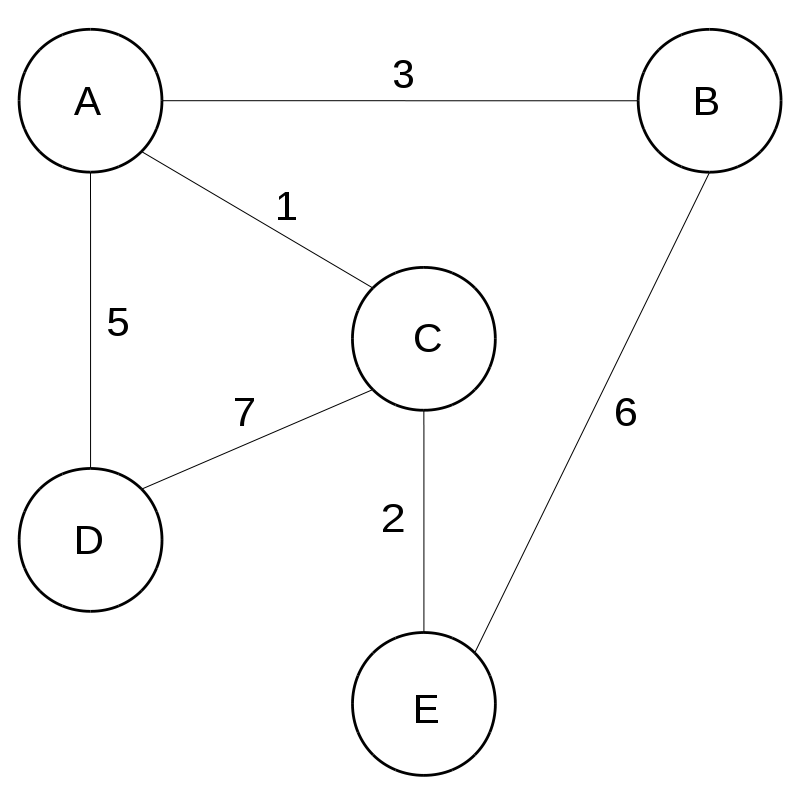
\includegraphics[width=12cm]{grafo.png}
\caption{Um grafo com 5 nós e 6 arestas.}
\label{fig:grafo}
\end{figure}

Quando a relação entre dois nós é simétrica, ou seja, a relação entre o nó $A$ e o nó $B$ é idêntica, diz-se que o grafo é \emph{não orientado}. Quando a relação entre dois nós é assimétrica, portanto, $A$ tem uma relação com $B$, mas essa relação não equivale a $B$ para $A$, tem-se um \emph{dígrafo} ou um \emph{grafo orientado}.

Este trabalho utiliza o grafo não orientado pois este bem representa as relações de amizade recíprocas. Tal decisão é tomada pois, quando da sugestão de um novo contato, ambos vão ser apresentados reciprocamente, estabelecendo, portanto, uma relação mútua de interação.

Diversas áreas da ciência, desde a biologia à linguística, utilizam grafos para representar dados. A representação de objetos e suas relações é uma ferramenta frequente em várias pesquisas.

Na ciência da computação, o grafo é a uma estrutura de dados amplamente frequente e existem centenas de problemas computacionais definidos com o seu uso \cite{Cormen2009}. Um caso tradicional com solução utilizando grafos é a do caixeiro viajante. Neste problema, os nós do grafo são as localidades e as arestas têm o peso equivalente à distância entre as cidades. \citep{Dijkstra1959}, propôs o primeiro algoritmo para encontrar o caminho mais curto entre dois nós de um grafo. O algoritmo encontra um caminho curto, mas não o ideal. Vários trabalhos são realizados ainda hoje na busca pelo caminho mais curto ideal em um grafo. Muitos desses trabalhos são baseados no algoritmo de Dijkstra. Esse algoritmo será apresentado ainda neste capítulo.

Como estrutura de dados computacionais, existem várias modelagens conhecidas para representação de um grafo. \citep{Cormen2009}, cita duas formas fundamentais:

\begin{itemize}
\item A lista de adjacência
\item A matriz de adjacência
\end{itemize}

\begin{figure}[!htb]
\centering
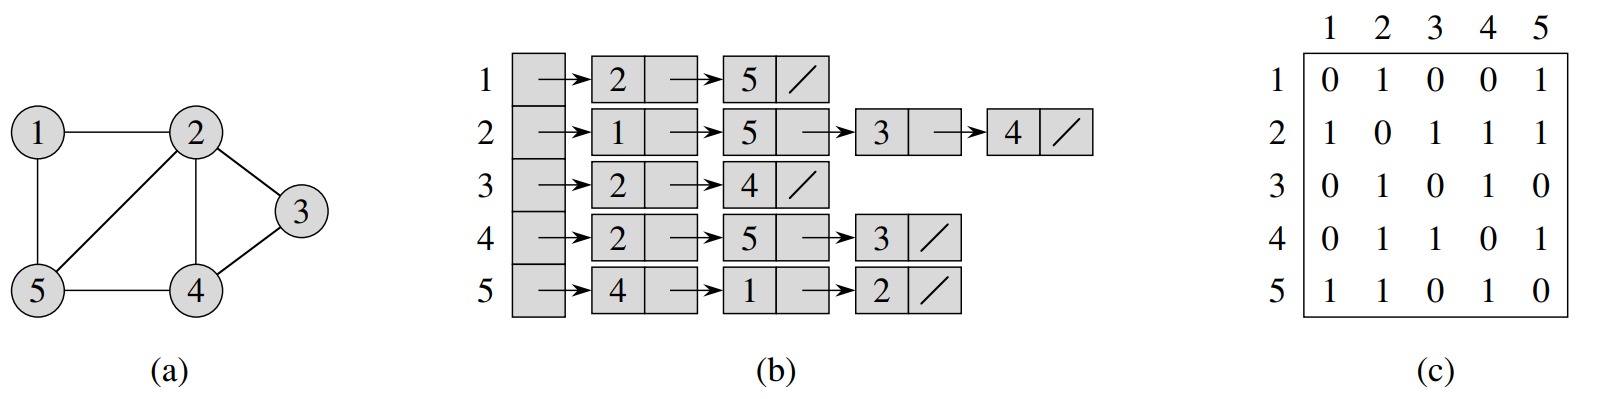
\includegraphics[width=16cm]{represent_grafo.png}
\caption{Duas representações de um grafo não direcionado. (\textbf{a}) Um grafo G com cinco nós e sete arestas. (\textbf{b}) A representação de uma lista de adjacência de G. (\textbf{c}) A representação de uma matriz de adjacência. Fonte: \cite{Cormen2009}, tradução dos autores.}
\label{fig:represent_grafo}
\end{figure}


\begin{figure}[!htb]
\centering
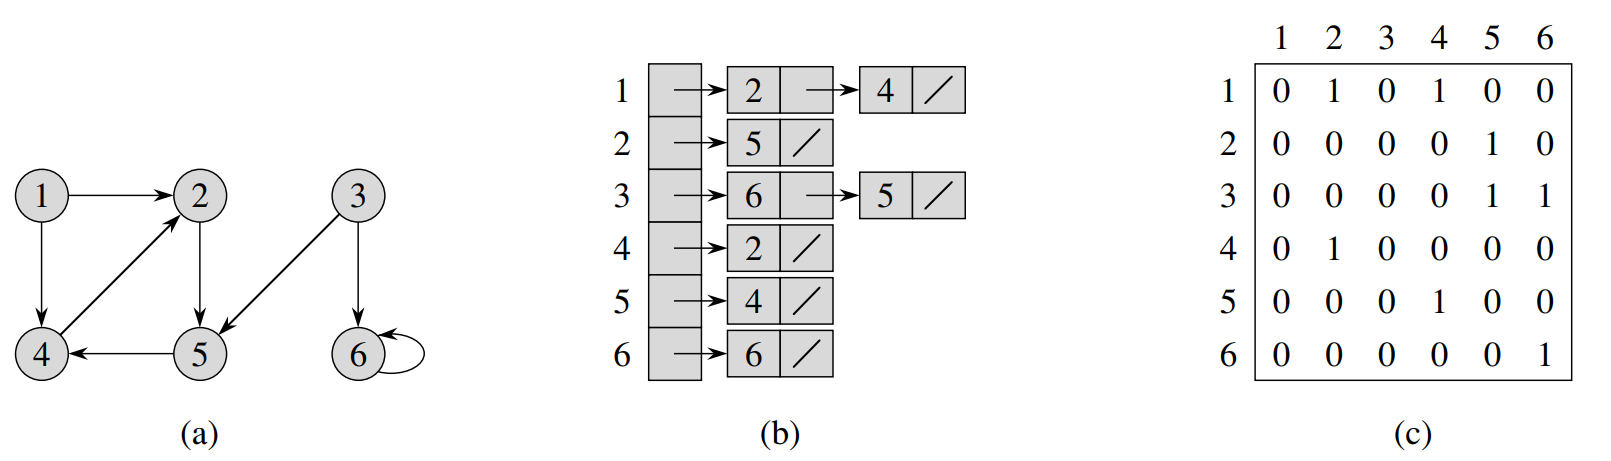
\includegraphics[width=16cm]{represent_grafo_ND.png}
\caption{Duas representações de um grafo direcionado. (\textbf{a}) Um grafo G com seis nós e oito arestas. (\textbf{b}) A representação de uma lista de adjacência de G. (\textbf{c}) A representação de uma matriz de adjacência. Fonte: \cite{Cormen2009}, tradução dos autores.}
\label{fig:represent_grafo_ND}
\end{figure}

A figura \ref{fig:represent_grafo}, ilustra um grafo G como um diagrama, como uma lista e como uma matriz. A implementação computacional das estruturas lista e matriz




The adjacency-list representation of a graph G = (V, E) consists of an array Adj of |V| lists, one for each vertex in V. For each u e V, the adjacency list Adj[u] contains all the vertices v such that there is an edge (u, v) e E. That is, Adj[u] consists of all the vertices adjacent to u in G. (Alternatively, it may contain pointers to these vertices.) The vertices in each adjacency list are typically stored in an arbitrary order. Figure 22.1(b) is an adjacency-list representation of the undirected graph in Figure 22.1(a). Similarly, Figure 22.2(b) is an adjacency-list representation of the directed graph in Figure 22.2(a). If G is a directed graph, the sum of the lengths of all the adjacency lists is |E|, since an edge of the form (u, v) is represented by having v appear in Adj[u]. If G is an undirected graph, the sum of the lengths of all the adjacency lists is 2 |E|, since if (u, v) is an undirected edge, then u appears in v’s adjacency list and vice versa. 22.1 Representations of graphs 529 For both directed and undirected graphs, the adjacency-list representation has the desirable property that the amount of memory it requires is 
(V + E). Adjacency lists can readily be adapted to represent weighted graphs, that is, graphs for which each edge has an associated weight, typically given by a weight function w : E → R. For example, let G = (V, E) be a weighted graph with weight function w. The weight w(u, v) of the edge (u, v) e E is simply stored with vertex v in u’s adjacency list. The adjacency-list representation is quite robust in that it can be modified to support many other graph variants. A potential disadvantage of the adjacency-list representation is that there is no quicker way to determine if a given edge (u, v) is present in the graph than to search for v in the adjacency list Adj[u]. This disadvantage can be remedied by an adjacency-matrix representation of the graph, at the cost of using asymptotically more memory. (See Exercise 22.1-8 for suggestions of variations on adjacency lists that permit faster edge lookup.) For the adjacency-matrix representation of a graph G = (V, E), we assume that the vertices are numbered 1, 2,...,|V| in some arbitrary manner. Then the adjacency-matrix representation of a graph G consists of a |V| x |V| matrix A = (aij) such that aij =  1 if (i, j)  E , 0 otherwise . Figures 22.1(c) and 22.2(c) are the adjacency matrices of the undirected and directed graphs in Figures 22.1(a) and 22.2(a), respectively. The adjacency matrix of a graph requires 
(V2) memory, independent of the number of edges in the graph. Observe the symmetry along the main diagonal of the adjacency matrix in Figure 22.1(c). We define the transpose of a matrix A = (aij) to be the matrix AT = (aT ij) given by aT ij = aji. Since in an undirected graph, (u, v) and (v, u) represent the same edge, the adjacency matrix A of an undirected graph is its own transpose: A = AT. In some applications, it pays to store only the entries on and above the diagonal of the adjacency matrix, thereby cutting the memory needed to store the graph almost in half. Like the adjacency-list representation of a graph, the adjacency-matrix representation can be used for weighted graphs. For example, if G = (V, E) is a weighted graph with edge-weight function w, the weight w(u, v) of the edge (u, v) e E is simply stored as the entry in row u and column v of the adjacency matrix. If an edge does not exist, a NIL value can be stored as its corresponding matrix entry, though for many problems it is convenient to use a value such as Although the adjacency-list representation is asymptotically at least as efficient as the adjacency-matrix representation, the simplicity of an adjacency matrix may make it preferable when graphs are reasonably small. Moreover, if the graph is unweighted, there is an additional advantage in storage for the adjacency-matrix 530 Chapter 22 Elementary Graph Algorithms representation. Rather than using one word of computer memory for each matrix entry, the adjacency matrix uses only one bit per entry.

